\section{Results}
\vspace{1cm}
We compare five generative priors against the LASSO baseline. Four of them are the models described in the previous section, a VAE and a DCGAN each trained with a latent vector of dimension 20 and 30. The fifth is the fully connected architecture of Bora et al. \cite{bora2017}, included so that the comparison with the numbers they publish is direct rather than indirect.

\subsection{Experimental Protocol}

Every method is evaluated on the same ten test images, one for each digit class, so that the comparison is not driven by a single lucky or unlucky example. At each measurement budget \( M \) the six methods receive the same measurement matrix \( A \) and the same noise vector, and the noise is scaled so that its expected norm remains equal to 0.1 whatever the value of \( M \).
\\
The reconstruction quality is measured as the squared distance between the reconstruction and the original image, divided by the number of pixels:
\begin{equation}
\text{error per pixel} = \frac{\lVert \hat{x} - x^* \rVert_2^2}{n}, \qquad n = 784 .
\end{equation}
This is not the same quantity as the measurement error \( \lVert AG(\hat{z}) - y \rVert \) that the recovery algorithm minimizes. The latter decreases as \( M \) decreases, simply because fewer constraints have to be satisfied, so it describes how well the optimization converged rather than how good the reconstruction is. For this reason it is used only as a diagnostic and to rank the random restarts, while every number reported below is computed against the ground truth image.
\\
All the reconstructions obtained with a generative prior use a thousand gradient steps, ten random restarts and the regularization weight \( \lambda = 0.1 \) recommended in \cite{bora2017}. Section 6.6 reports what happens without the regularization term.

\subsection{Baseline Performance Using LASSO}

We started by evaluating the baseline performance using LASSO for reconstruction. LASSO (Least Absolute Shrinkage and Selection Operator) assumes sparsity in the signal and solves the following optimization problem:
\begin{equation}
\hat{x} = \arg \min_x \|y - Ax\|_2^2 + \alpha \|x\|_1,
\end{equation}
\\
where \( y \) is the measurement vector, \( A \) is the measurement matrix, and \( \alpha \) is a regularization parameter. We solve it in an orthonormal DCT basis, which is the domain in which MNIST digits are compressible.
\\
From our experiments, we observed that the performance of LASSO is inadequate until a substantial number of measurements is available. Below 100 measurements the reconstruction is dominated by background noise, and a coherent digit only emerges from about 200 measurements onwards. On the other hand LASSO keeps improving as measurements are added, and it becomes the most accurate method of all once the budget is large.

\subsection{Comparison of the Six Methods}

Table \ref{tab:results} and figure \ref{fig:error vs measurements} report the error per pixel of every method as the number of measurements grows.

\begin{table}[H]
    \centering
    \small
    \begin{tabular}{r|cccccc}
    \( M \) & LASSO & VAE (paper) & VAE \( k{=}20 \) & VAE \( k{=}30 \) & DCGAN \( k{=}20 \) & DCGAN \( k{=}30 \) \\
    \hline
    10  & 0.1539 & 0.0609 & 0.0635 & 0.0766 & 0.1021 & 0.0833 \\
    25  & 0.1049 & 0.0291 & 0.0372 & \textbf{0.0225} & 0.0619 & 0.0465 \\
    50  & 0.0850 & \textbf{0.0110} & 0.0131 & 0.0177 & 0.0430 & 0.0347 \\
    75  & 0.0707 & \textbf{0.0079} & 0.0111 & 0.0094 & 0.0248 & 0.0319 \\
    100 & 0.0560 & \textbf{0.0076} & 0.0106 & 0.0080 & 0.0137 & 0.0291 \\
    200 & 0.0366 & \textbf{0.0067} & 0.0097 & 0.0077 & 0.0106 & 0.0235 \\
    300 & 0.0206 & \textbf{0.0066} & 0.0096 & 0.0074 & 0.0105 & 0.0247 \\
    400 & 0.0117 & \textbf{0.0066} & 0.0096 & 0.0074 & 0.0098 & 0.0223 \\
    500 & \textbf{0.0065} & 0.0066 & 0.0096 & 0.0074 & 0.0094 & 0.0238 \\
    750 & \textbf{0.0015} & 0.0064 & 0.0094 & 0.0072 & 0.0095 & 0.0225 \\
    \end{tabular}
    \caption{Error per pixel, averaged over ten test digits, one per class. The best method at each budget is in bold. VAE (paper) is the fully connected architecture of \cite{bora2017}.}
    \label{tab:results}
\end{table}

\begin{figure}[H]
    \centering
    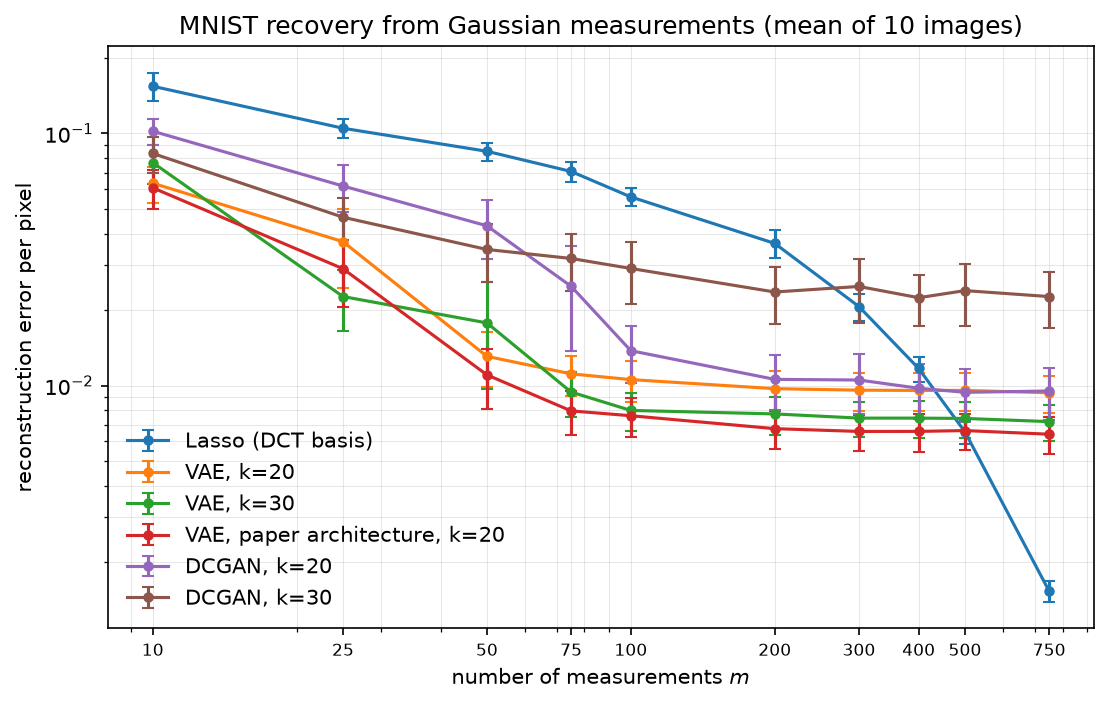
\includegraphics[width=1\linewidth]{assets/error_vs_measurements.png}
    \caption{Error per pixel as a function of the number of measurements \( M \). Bars are standard errors over the ten test images. Both axes are logarithmic.}
    \label{fig:error vs measurements}
\end{figure}

Three regimes can be distinguished.
\\\\
\textbf{Few measurements.} Up to about one hundred measurements every generative prior is far more accurate than LASSO. With 25 measurements the best model has an error of 0.0225 against 0.1049 for LASSO, a factor 4.7, and at that budget the LASSO reconstruction is not recognizable as a digit at all. This is the regime that motivates compressed sensing, and it is where the choice of the prior matters most.
\\\\
\textbf{Sample efficiency.} LASSO needs 400 measurements to reach an error of 0.0117. The architecture of the reference paper reaches the same level with 50 measurements, a saving of a factor \textbf{8}, and our convolutional VAEs with 75 measurements, a factor 5.3. The DCGAN with latent dimension 20 needs 200, a factor 2. Bora et al. report a saving between 5 and 10 times, and our reproduction of their architecture falls inside that interval.
\\\\
\textbf{Many measurements.} From 500 measurements onwards LASSO becomes the most accurate method and keeps improving, reaching 0.0015 with 750 measurements against 0.0064 for the best generative model, a reversal by a factor 4.3. This behaviour is expected and is described in \cite{bora2017}, where the authors observe that LASSO eventually surpasses the generative approach and that this requires more than 500 measurements. Our experiment reproduces that threshold.
\\\\
The reason for the reversal is that the reconstruction is constrained to lie in the range of the generator. The distance between a real digit and that range does not depend on the number of measurements, so once enough measurements are available to identify the closest point in the range, additional measurements bring no benefit. Averaging the budgets from 300 upwards, this residual error settles at 0.0065 for the paper architecture, 0.0074 for the VAE with latent dimension 30, 0.0095 for the VAE with latent dimension 20, 0.0098 for the DCGAN with latent dimension 20 and 0.0233 for the DCGAN with latent dimension 30. These five values are properties of the generators and not of the recovery algorithm.

\subsection{Reconstruction Examples}

Figure \ref{fig:reconstruction grid} shows the same digit reconstructed by every method at every budget.

\begin{figure}[H]
    \centering
    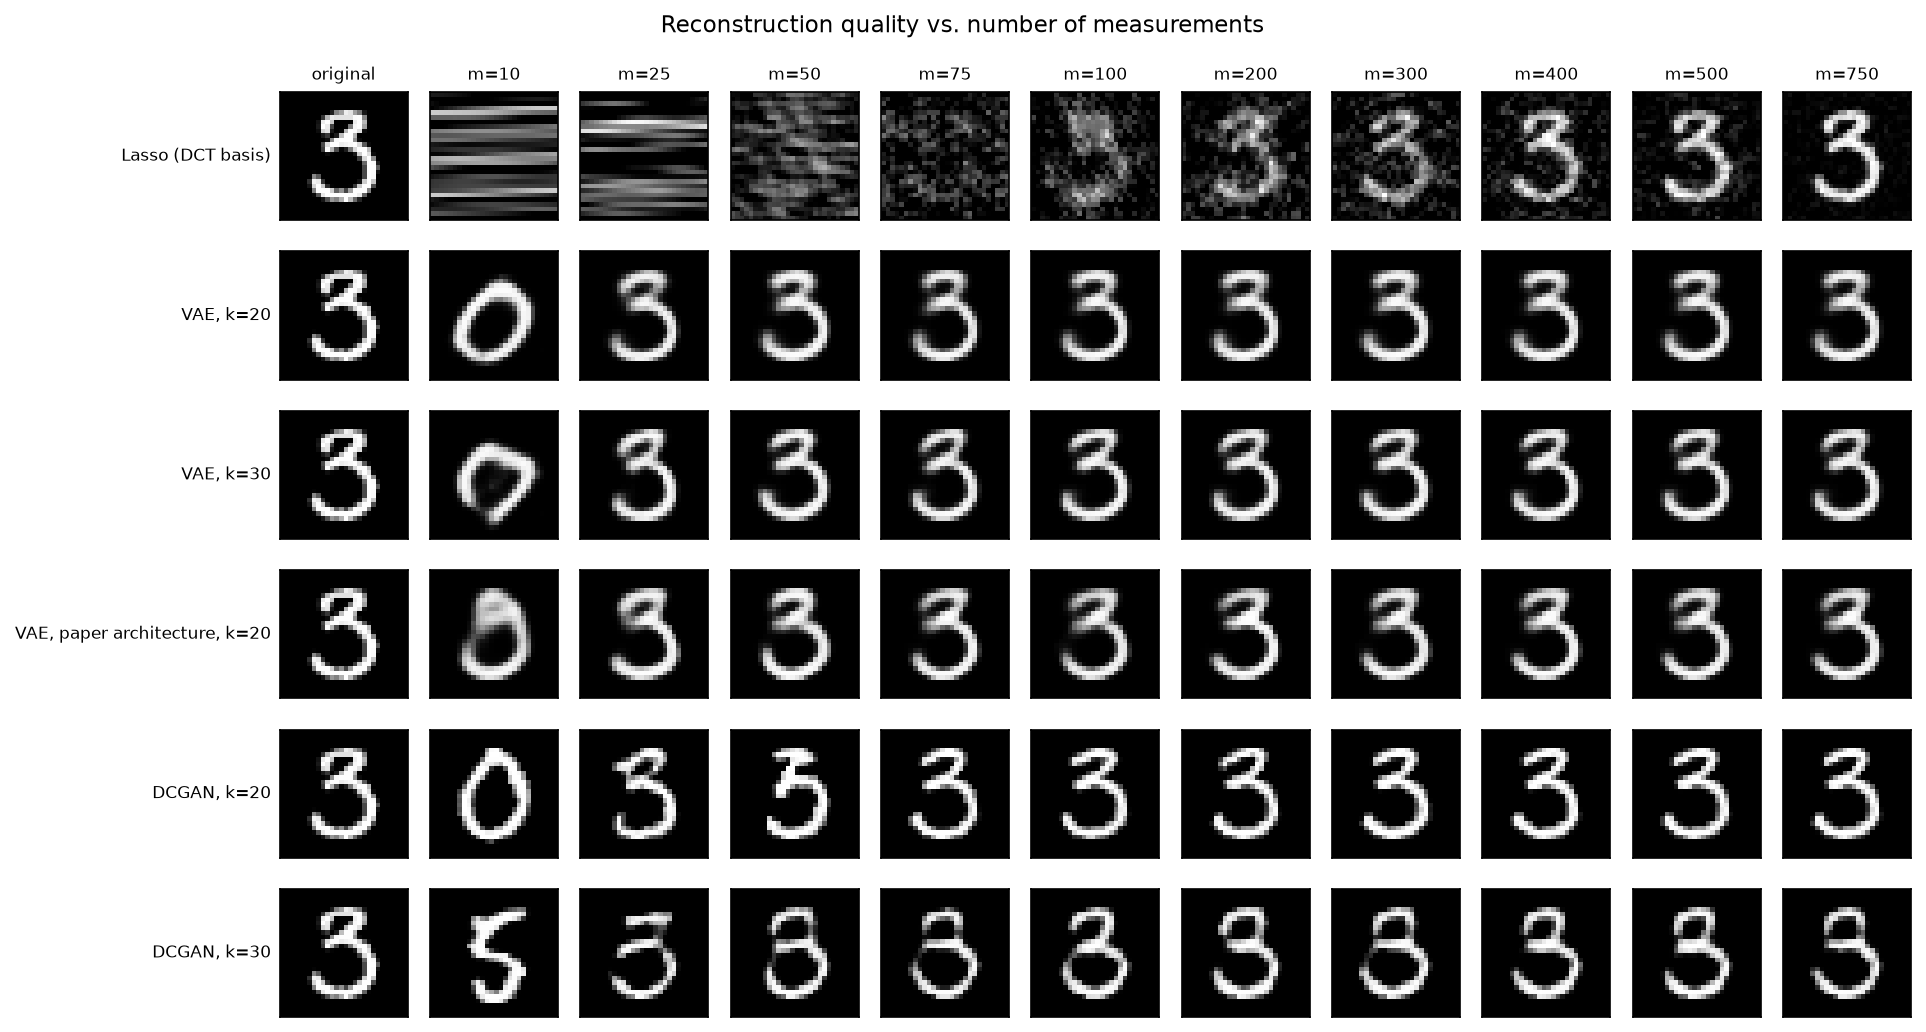
\includegraphics[width=1\linewidth]{assets/reconstruction_grid.png}
    \caption{One test digit reconstructed by the six methods as the number of measurements increases}
    \label{fig:reconstruction grid}
\end{figure}

The visual comparison confirms the numbers. LASSO returns noise until about 200 measurements, while the generative priors produce a plausible digit almost immediately. The DCGAN gives visibly sharper strokes than the VAE, which is consistent with the fact that an adversarial generator is trained to produce samples a discriminator accepts, rather than an average of the plausible reconstructions as the VAE does. Sharpness and accuracy are not the same thing, however, and as the table shows the sharper model is also the less accurate one.

\subsection{Architecture and Latent Dimension}

Because every method sees the same images and the same measurement matrices, the comparisons below are paired, and we test them with a paired t-test over the ten images at each budget.
\\\\
\textbf{The architecture of the paper outperforms ours.} With the same latent dimension of 20, the fully connected network of \cite{bora2017} is more accurate than our convolutional VAE at every budget, and the difference is significant from 75 measurements upwards, with p-values between 0.003 and 0.001 and an advantage on 9 of the 10 test images. Below 75 measurements the difference is not significant. This is a result we did not expect, since the convolutional architecture is the more sophisticated of the two, and it suggests that what matters for this task is how faithfully the generator covers the data manifold rather than how well suited its architecture is to images.
\\\\
\textbf{A larger latent space helps, but only past the low measurement regime.} For the convolutional VAE, the version with \( k = 30 \) is more accurate than the one with \( k = 20 \) from 75 measurements upwards, with p-values between 0.028 and 0.003 and an advantage on 9 of the 10 images. At 10, 25 and 50 measurements the difference is not significant and its sign is not even stable. This matches the intuition that a larger latent space represents digits more faithfully, which lowers the error floor, but offers no advantage while the measurements are too few to determine the extra coordinates.
\\\\
\textbf{The VAE beats the DCGAN where measurements are scarce.} At 10 and 50 measurements the convolutional VAE is significantly more accurate than the DCGAN of the same latent dimension, with p-values of 0.011 and 0.024. From 200 measurements onwards the two are indistinguishable, and both have settled on their respective floors.

\subsection{The Latent Regularizer}

Figure \ref{fig:regularisation} compares the results obtained with \( \lambda = 0.1 \) and with the term removed.

\begin{figure}[H]
    \centering
    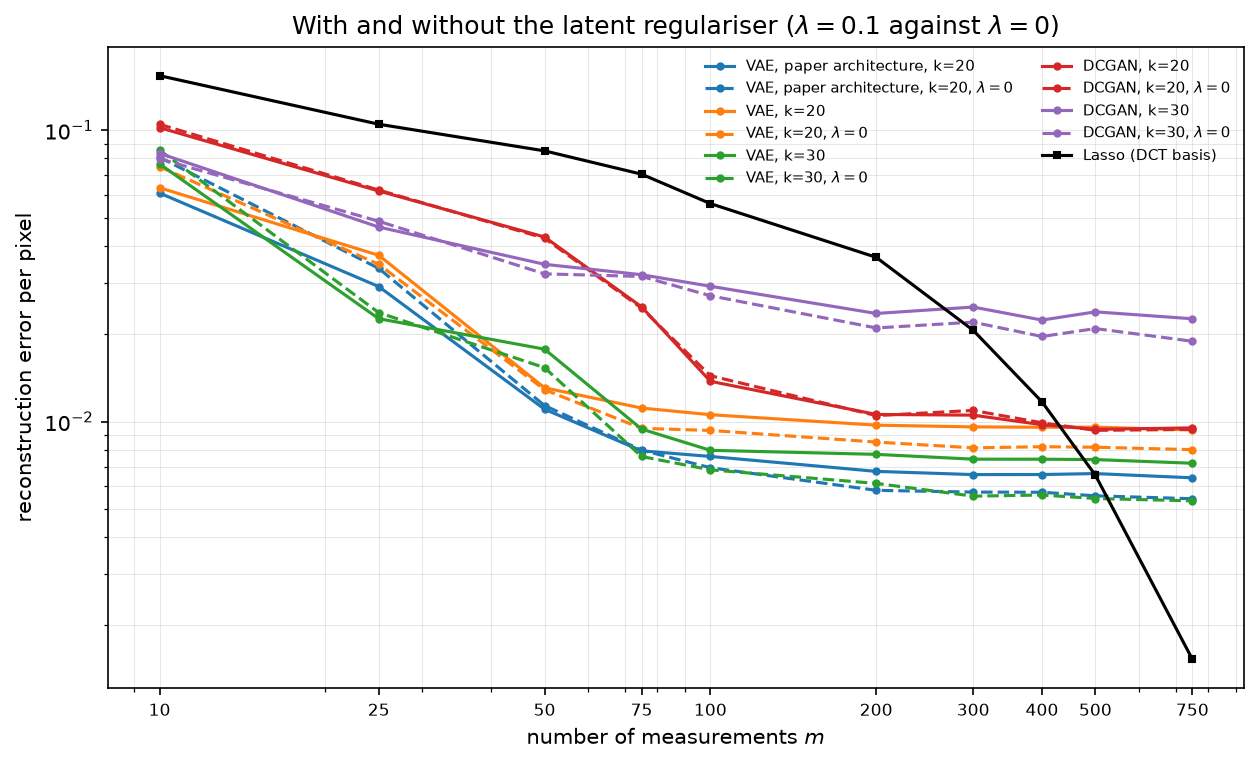
\includegraphics[width=1\linewidth]{assets/regularisation_comparison.png}
    \caption{Recovery with and without the latent regularization term}
    \label{fig:regularisation}
\end{figure}

The term behaves as its motivation suggests. It helps when the measurements are few, where the data alone does not determine the latent vector and the prior supplies the missing information: with 10 measurements the error of the paper architecture falls from 0.0808 to 0.0609, an improvement of 25\%. It is mildly harmful once measurements are plentiful, where the same pull towards the prior keeps the solution from reaching the closest point in the range of the generator: with 750 measurements the error rises from 0.0054 to 0.0064.
\\
A sweep over \( \lambda \in \{0, 0.01, 0.1, 1\} \) confirms the mechanism directly. The norm of the recovered latent vector falls monotonically with \( \lambda \), from 7.7 to 2.5 for the paper architecture, so the term does constrain the search as intended, and the reconstruction error is lowest for intermediate values and worsens again at \( \lambda = 1 \), where the pull towards the origin dominates the measurements.

\subsection{Computational Cost}

The methods are not comparable in cost. Reconstructing the ten test images at one budget, with ten restarts and a thousand gradient steps, takes on average 1.0 seconds with LASSO, 6.8 seconds with the fully connected decoder of the paper, about 15 seconds with our convolutional decoders and about 496 seconds with a DCGAN generator. The factor 73 between the cheapest and the most expensive generative prior is explained by the size of the generator, since the DCGAN generator has 2.9 million parameters against 0.65 million for the fully connected one and ends with a transposed convolution producing 512 feature maps at full resolution. The complete experiment reported in this section required 2.9 hours of computation.
\\
This cost is incurred at every reconstruction and not only once during training, because recovery is itself an optimization problem. It is worth stressing that the most expensive prior is also the least accurate one, so on this dataset there is no trade-off to arbitrate between the two.

\subsection{Reproducibility of the Training}

While preparing these results we found that training the same VAE with the same script and different random seeds produced generators of very different quality. Measured as the best reconstruction reachable inside the range of the generator, the results ranged from 0.0103 to 0.0358 for \( k = 30 \), a factor of 3.5, which is larger than any difference between the models we set out to compare.
\\
The cause is partial posterior collapse: in the weaker runs the decoder relies on a few latent directions and ignores the rest. Measuring how much each latent coordinate moves the generated image, the ratio between the average sensitivity and the largest one is 0.31 for the best model and 0.05 for the worst, and that ratio orders the models exactly as the reconstruction error does.
\\
Adding a KL warm-up, as described in section 3.2.3, removes the problem. The spread across seeds falls from a factor 3.5 to about 20\%, the KL divergence at convergence rises from between 4 and 7 nats to between 16 and 23, and the resulting models are better than any obtained without it. The checkpoints used in this section were selected on validation loss alone, following a procedure fixed before the runs were carried out and recorded in the repository.
\\
We report this because it affects how the comparisons above should be read: differences between priors are only meaningful when they are larger than the variability of the training procedure that produced them.
